% !TEX encoding = UTF-8
% !TEX TS-program = pdflatex
% !TEX root = ../tesi.tex
% !TEX spellcheck = it-IT

%**************************************************************
\chapter{Multiplatform File Analyzer}
\label{cap:multiplatform-file-analyzer}
%**************************************************************

\intro{In questo capitolo è presente una analisi completa del tool Multiplatform Fyle Analyzer}\\

\section{Introduzione}

	\subsection{Premessa}
		Tutti i giochi multipiattaforma prodotti da Milestone sono saggiamente organizzati in modo che ogni qual volta debbano ricercare un file dato un percorso, prima eseguono la ricerca nella cartella specifica della piattaforma di esecuzione e poi, se non presente, nel percorso originale dato\footnote{Lo stesso sistema è utilizzato anche per il caricamento dei file contenenti i testi specifici per ogni differente localizzazione del gioco.}. Grazie a questa organizzazione si riesce facilmente a differenziare gli asset in maniera molto semplice e veloce ogni qual volta sia necessario.\\
		La differenziazione degli asset nasce principalmente dalle differenti specifiche tecniche e capacità di calcolo di ciascuna piattaforma che costringono a creare versioni apposite. Ovviamente la specializzazione è un costo aggiuntivo in termini di tempo di creazione e di manutenzione e va eseguita il meno possibile.
		
	\subsection{Lo scopo}
		Inizialmente il metodo adottato funzionava senza problemi evidenti ma, al veloce crescere del numero dei file e delle piattaforme target\footnote{Le piattaforme target sono attualmente sei: \textit{Playstation Vita, Playstation 3, Xbox 360, Playstation 4 e Xbox One.}}, si è notata l'esigenza di avere un maggior controllo.\\
		Multiplaform File Analyzer è stato realizzato appositamente per rimediare a questo problema, offrendo una panoramica semplice ma completa riguardo le differenti versioni di ogni file specializzato per almeno una piattaforma.

\section{Casi d'uso}

	Per meglio capire e tracciare l'esperienza d'uso che un developer di un gioco multipiattaforma avrà con il tool sono stati creati dei diagrammi di casi d'uso gerarchici.\\
	I diagrammi di casi d'uso fanno parte della famiglia dei diagrammi UML e descrivono le funzionalità offerte dal prodotto così come sono percepite dagli attori che interagiscono con il sistema.\\
	Ogni caso d'uso ha un codice univoco gerarchico, nella forma:
	\begin{center} 
		UC[codice univoco del padre].[codice progressivo di livello]
	\end{center}
	\paragrafo Il codice progressivo può includere diversi livelli di gerarchia separati da un punto.
	
	\subsection{UC 1: Caso d'uso principale}
		\label{subsec:UC1}
	
		\begin{figure}[!h] 
			\centering 
			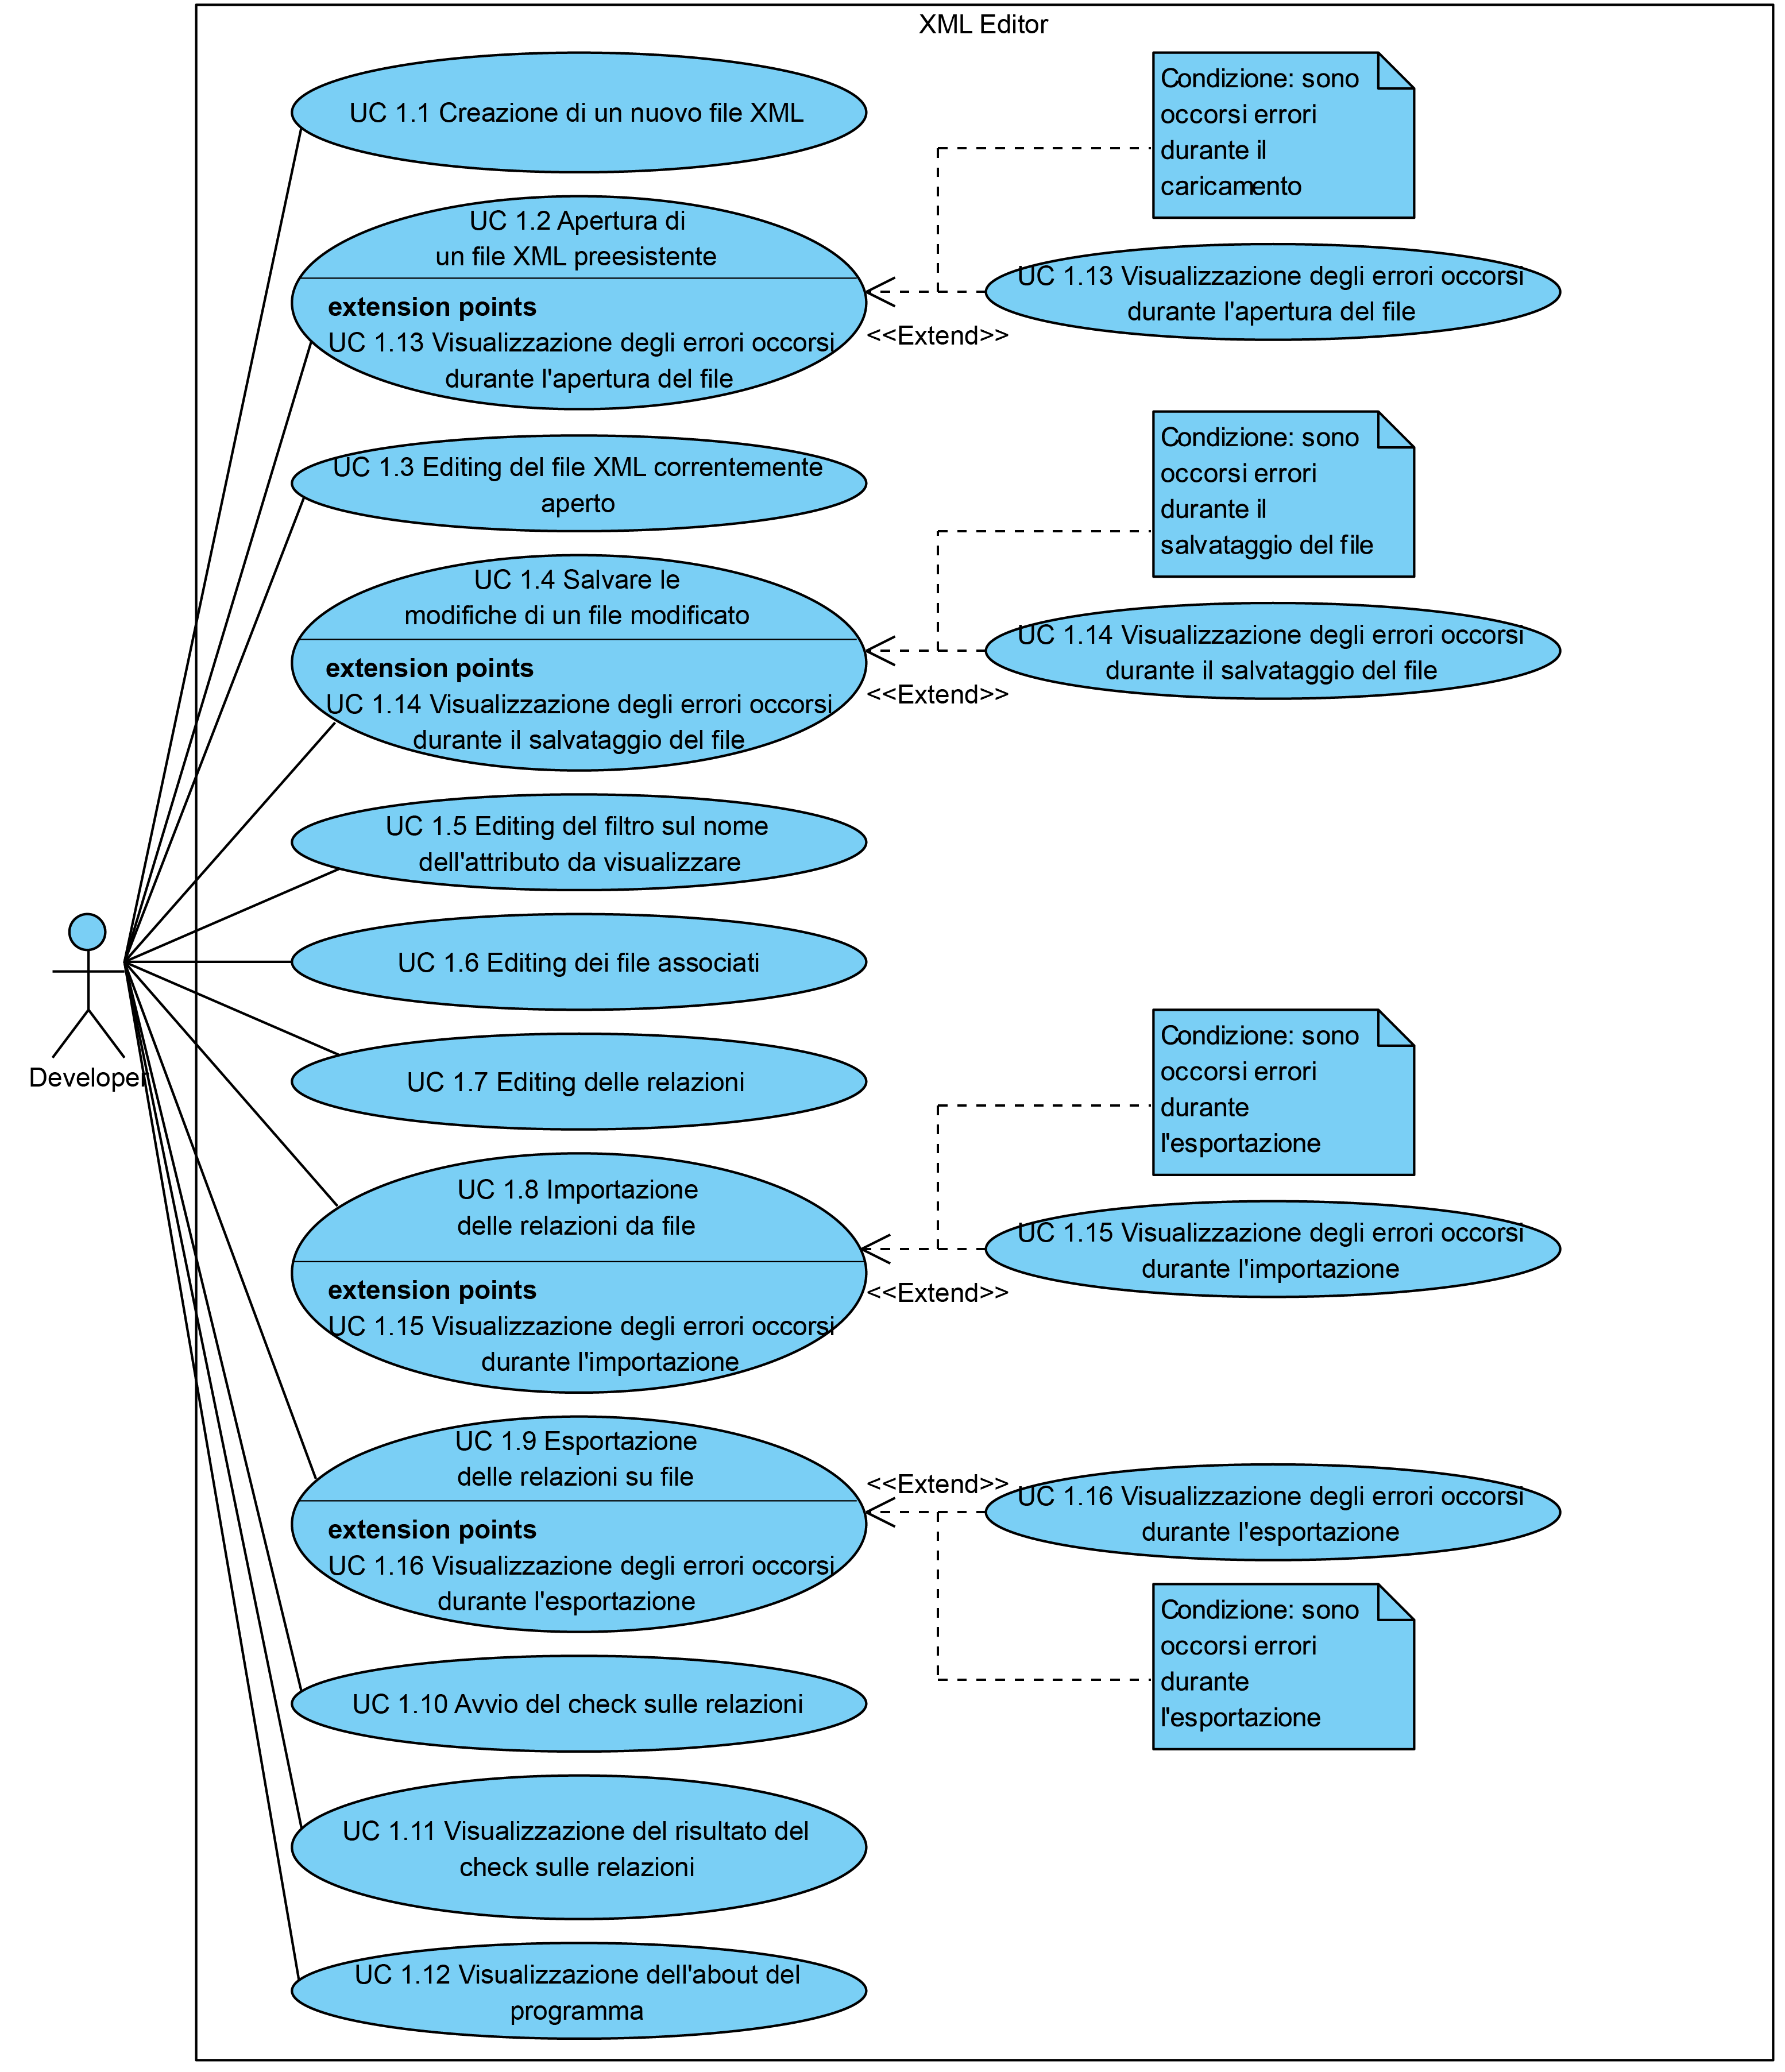
\includegraphics[width=0.9\columnwidth]{tool1/UC1.png} 
			\caption{Use Case - UC 1: Caso d'uso principale}
		\end{figure}
		
		\begin{itemize}
			\item\textbf{Attori}: developer.
			\item\textbf{Descrizione}: un developer può eseguire un'analisi dei file di un gioco multipiattaforma.
			\item\textbf{Precondizione}: il developer abbia lanciato il tool sotto un sistema Windows 7 o superiore.
			\item\textbf{Flusso principale degli eventi}: 
			\begin{enumerate}
				\item\textit{Analisi dei file di un gioco multipiattaforma} (\hyperref[subsec:UC1.1]{UC 1.1}).
			\end{enumerate}
			\item\textbf{Postcondizione}: il sistema ha erogato le funzionalità richieste dal developer.
		\end{itemize}
		
	\subsection{UC 1.1: Analisi dei file di un gioco multipiattaforma}
		\label{subsec:UC1.1}
		
		\begin{figure}[!h] 
			\centering 
			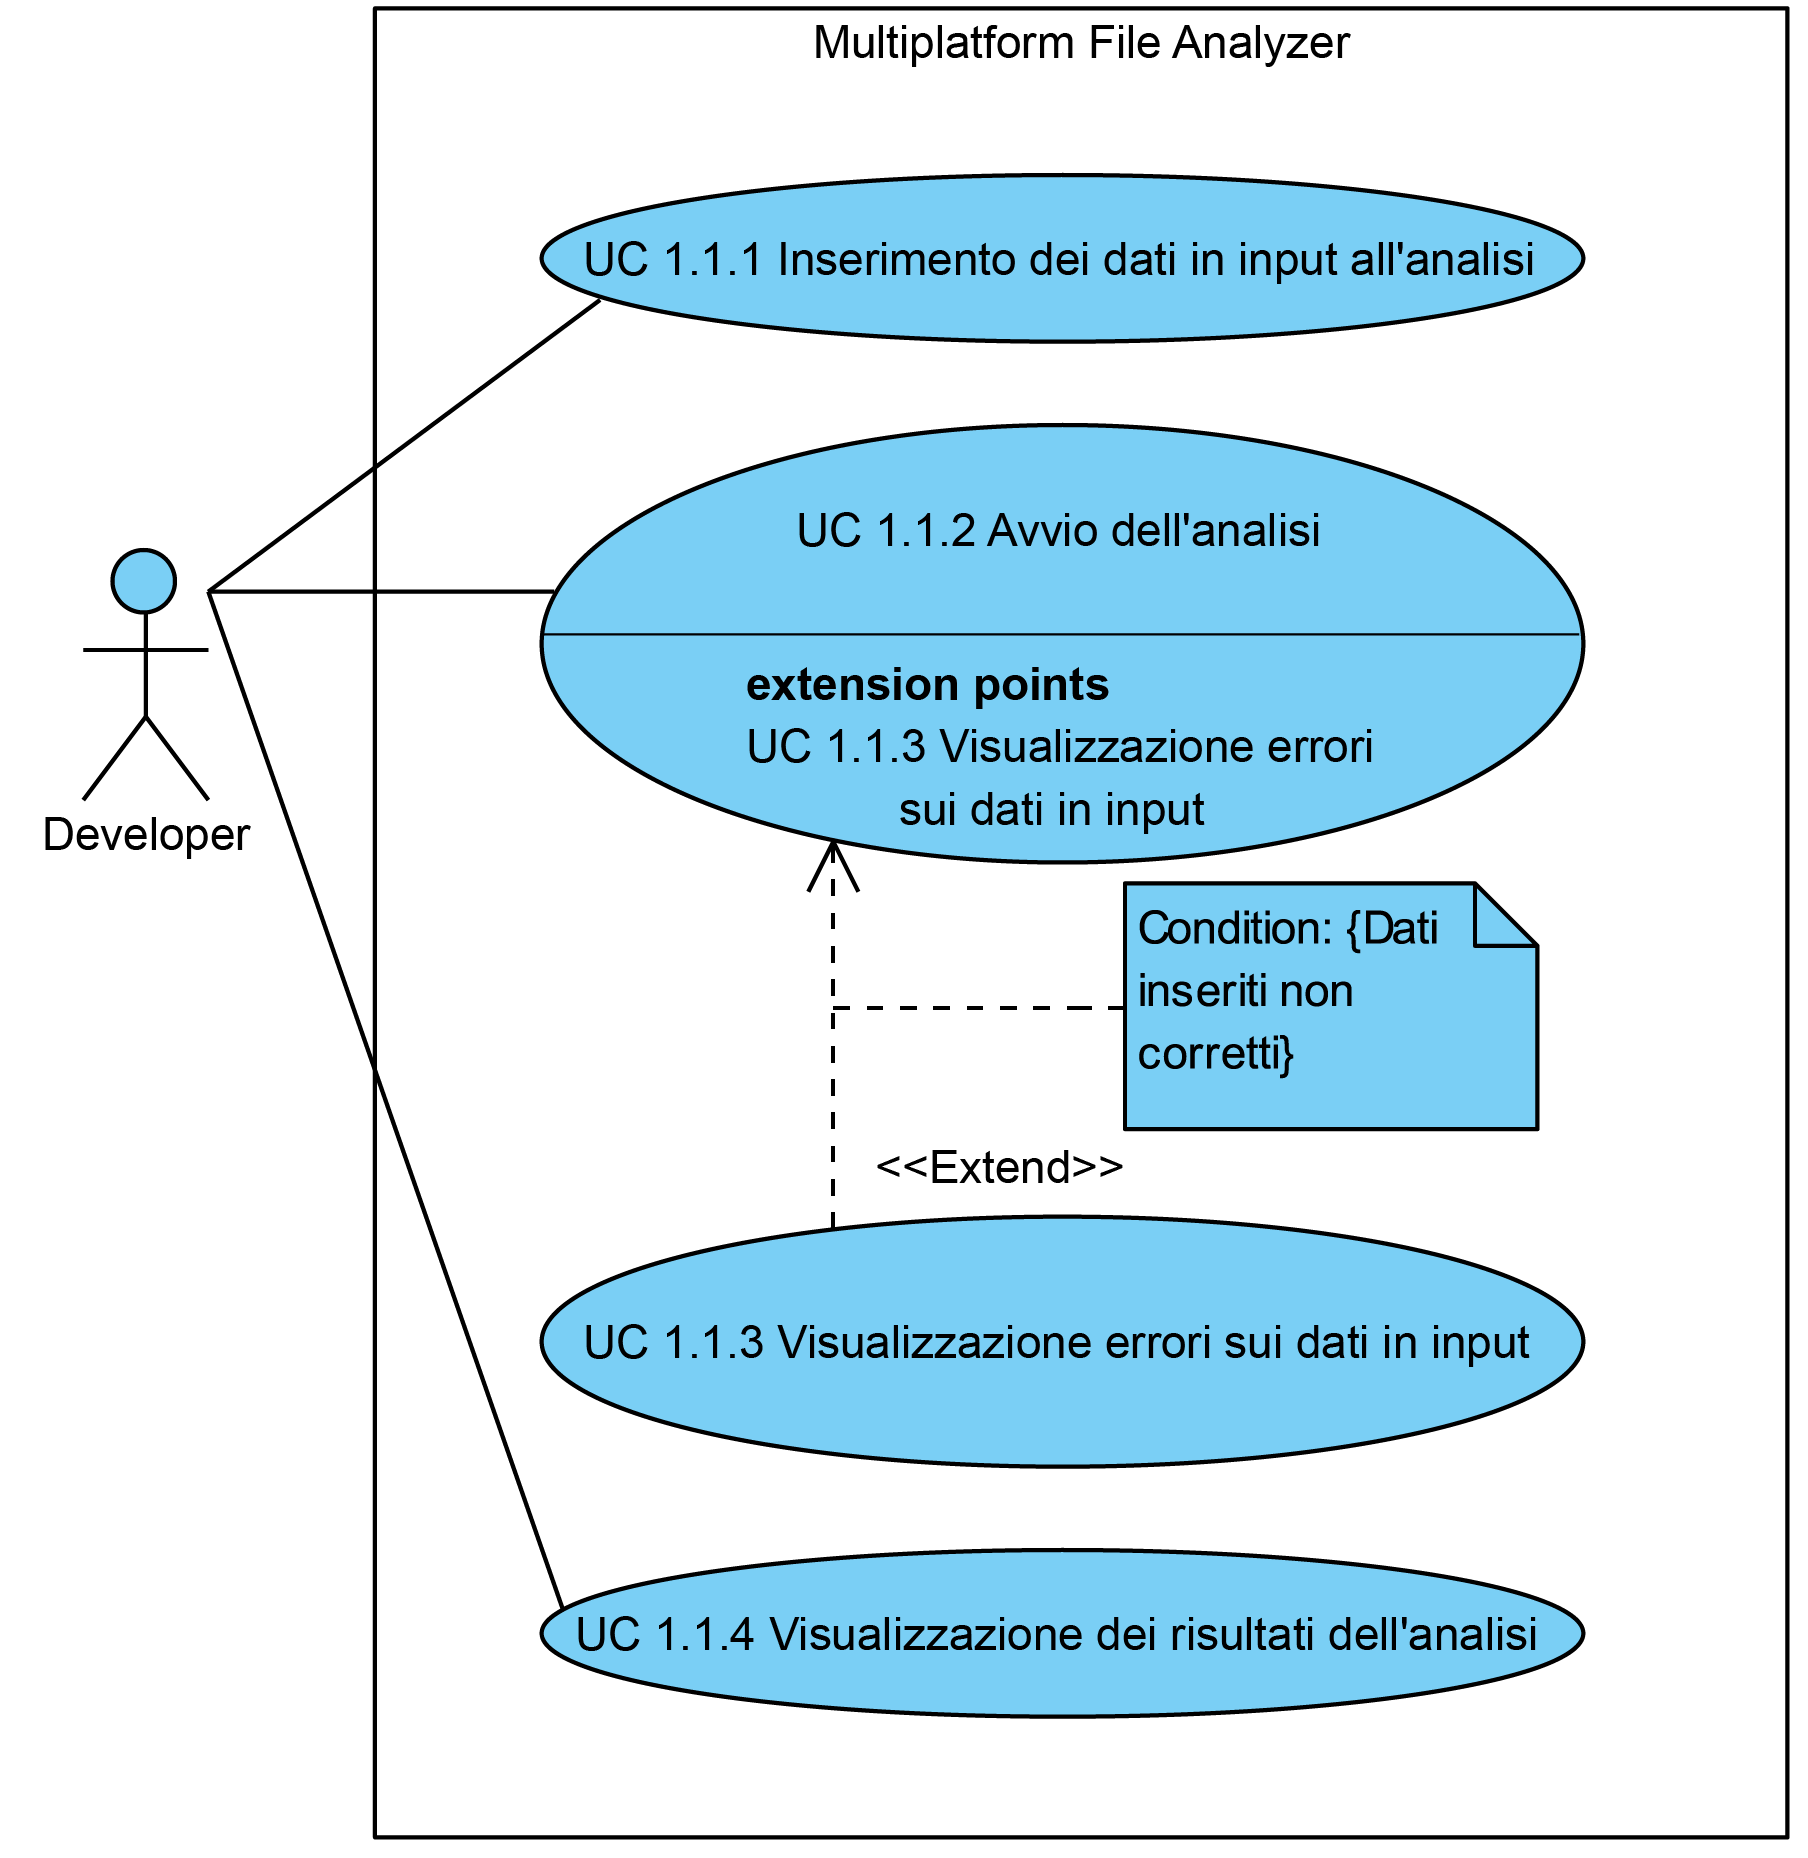
\includegraphics[width=0.9\columnwidth]{tool1/UC1-1.png} 
			\caption{Use Case - UC 1.1: Analisi dei file di un gioco multipiattaforma}
		\end{figure}
		
		\begin{itemize}
			\item\textbf{Attori}: developer.
			\item\textbf{Descrizione}: un developer deve poter inserire i dati necessari all'analisi, visualizzare eventuali errori oppure il risultato dell'analisi.
			\item\textbf{Precondizione}: il developer abbia lanciato il tool sotto un sistema Windows 7 o superiore.
			\item\textbf{Flusso principale degli eventi}: 
			\begin{enumerate}
				\item\textit{Inserimento dei dati in input all'analisi} (\hyperref[subsec:UC1.1.1]{UC 1.1.1});
				\item\textit{Avvio dell'analisi} (\hyperref[subsec:UC1.1.2]{UC 1.1.2});
				\item\textit{Visualizzazione del risultato dell'analisi} (\hyperref[subsec:UC1.1.4]{UC 1.1.4}).
			\end{enumerate}
			\item \textbf{Estensioni}
			\begin{enumerate}
				\item\textit{Visualizzazione errori sui dati in input} (\hyperref[subsec:UC1.1.3]{UC 1.1.3}).
			\end{enumerate}
			\item\textbf{Postcondizione}: il sistema ha erogato le funzionalità richieste dal developer.
		\end{itemize}
	
	\subsection{UC 1.1.1: Inserimento dei dati in input all'analisi}
		\label{subsec:UC1.1.1}
		
		\begin{figure}[!h] 
			\centering 
			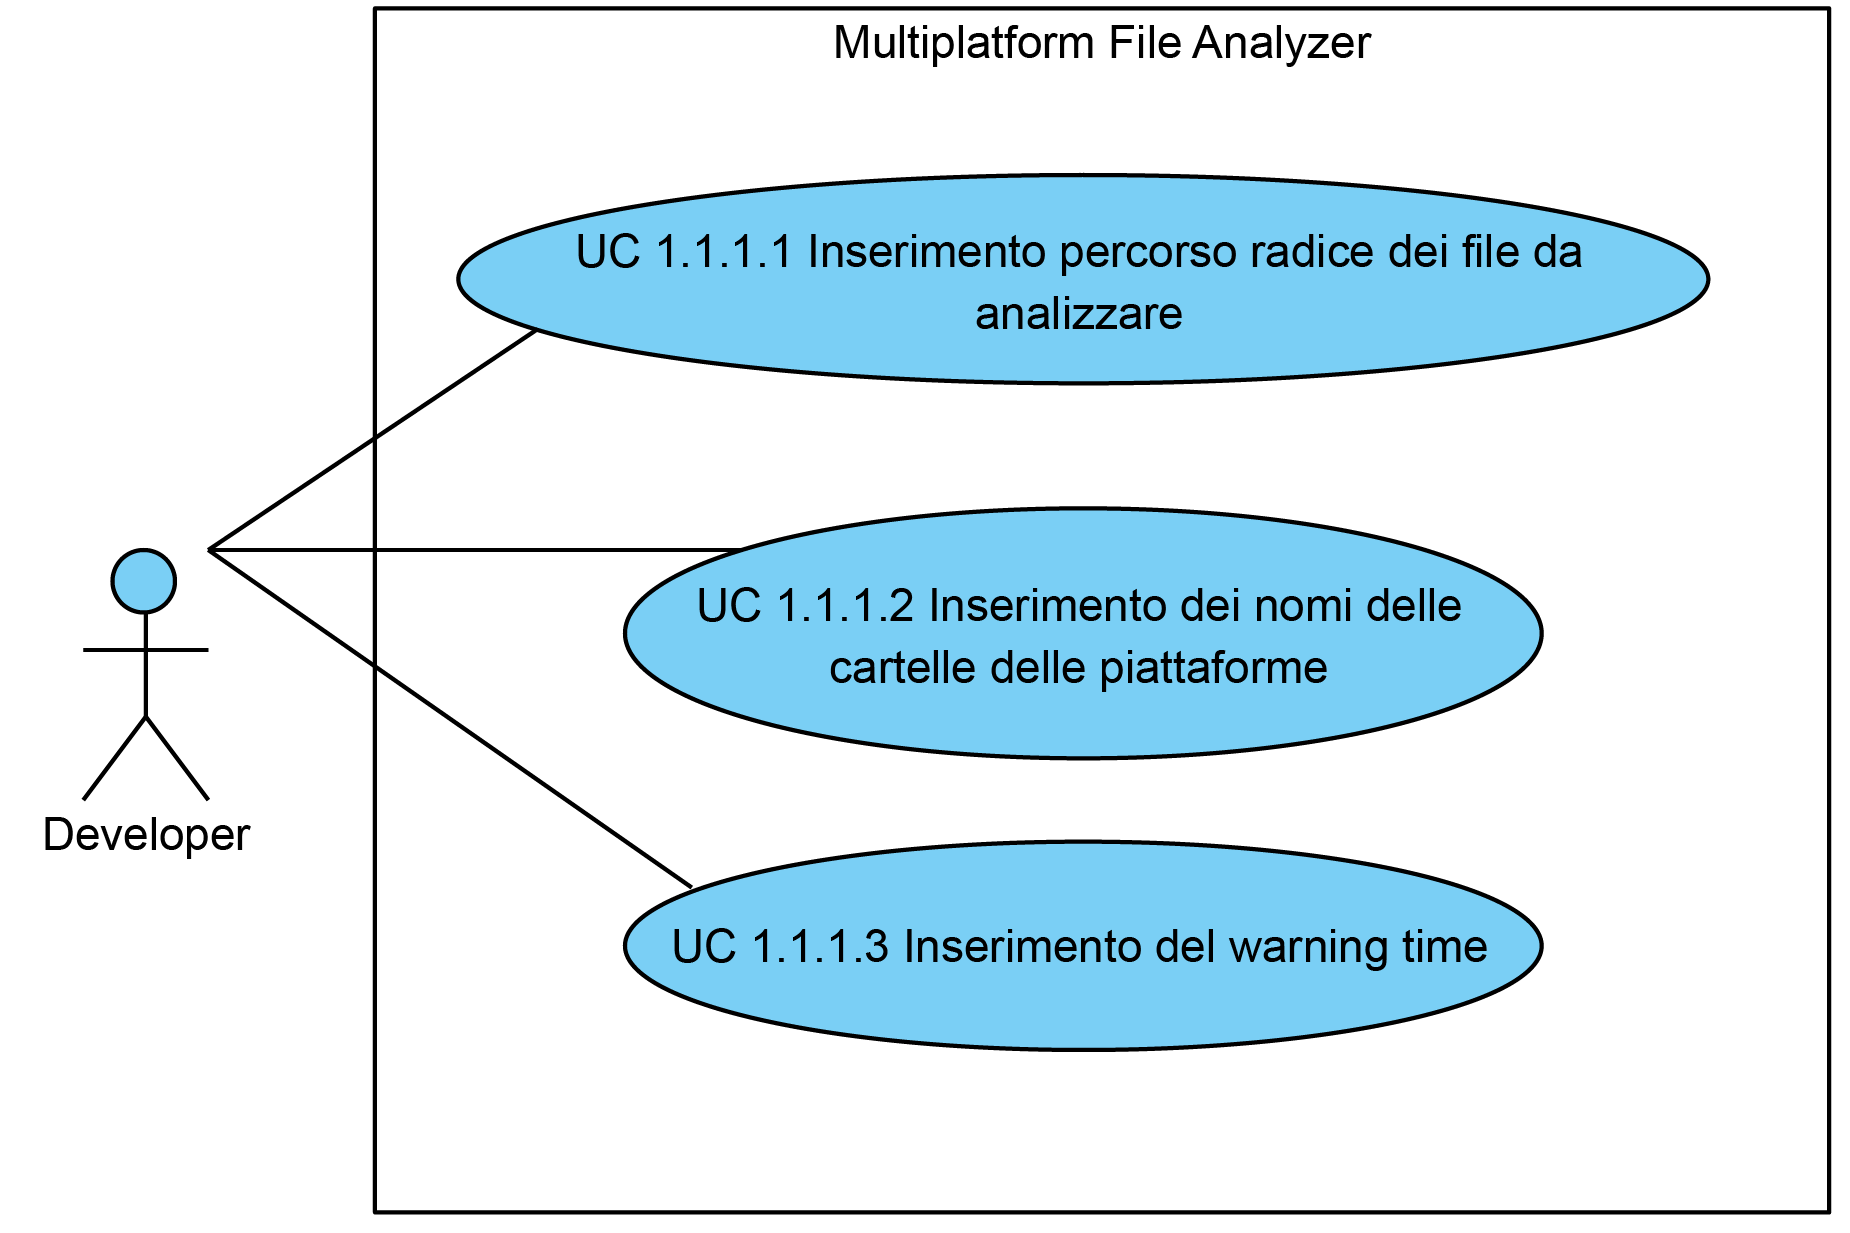
\includegraphics[width=0.9\columnwidth]{tool1/UC1-1-1.png} 
			\caption{Use Case - UC 1.1.1: Inserimento dei dati in input all'analisi}
		\end{figure}
		
		\begin{itemize}
			\item\textbf{Attori}: developer.
			\item\textbf{Descrizione}: un developer deve poter inserire i dati necessari all'analisi composti da un percorso di base, i nomi delle piattaforme e il tempo di warning.
			\item\textbf{Precondizione}: il developer abbia lanciato il tool sotto un sistema Windows 7 o superiore.
			\item\textbf{Flusso principale degli eventi}: 
			\begin{enumerate}
				\item\textit{Inserimento percorso radice dei file da analizzare} (\hyperref[subsec:UC1.1.1.1]{UC 1.1.1.1});
				\item\textit{Inserimento dei nomi delle cartelle delle piattaforme} (\hyperref[subsec:UC1.1.1.2]{UC 1.1.1.2});
				\item\textit{Inserimento del warning time} (\hyperref[subsec:UC1.1.1.3]{UC 1.1.1.3}).
			\end{enumerate}
			\item\textbf{Postcondizione}: il sistema ha preso in carico i dati che verranno usati per la prossima analisi.
		\end{itemize}
		
	\subsection{UC 1.1.1.1: Inserimento percorso radice dei file da analizzare}
		\label{subsec:UC1.1.1.1}
		
		\begin{itemize}
			\item\textbf{Attori}: developer.
			\item\textbf{Descrizione}: il developer deve poter inserire il percorso di base dell'analisi.
			\item\textbf{Precondizione}: il developer abbia lanciato il tool sotto un sistema Windows 7 o superiore.
			\item\textbf{Scenario principale}: il developer sceglie il percorso di base da cui l'analisi partirà.
			\item\textbf{Postcondizione}: il sistema ha preso in carico il percorso di base inserito che verrà usato per la prossima analisi.
		\end{itemize}

	\subsection{UC 1.1.1.2 Inserimento dei nomi delle cartelle delle piattaforme}
		\label{subsec:UC1.1.1.2}
	
		\begin{itemize}
			\item\textbf{Attori}: developer.
			\item\textbf{Descrizione}: il developer deve poter inserire i nomi delle piattaforme da analizzare.
			\item\textbf{Precondizione}: il developer abbia lanciato il tool sotto un sistema Windows 7 o superiore.
			\item\textbf{Scenario principale}: il developer sceglie i nomi delle piattaforme.
			\item\textbf{Postcondizione}: il sistema ha preso in carico i nomi delle piattaforme inserite che verranno usate per la prossima analisi.
		\end{itemize}
		
	\subsection{UC 1.1.1.3 Inserimento del warning time}
		\label{subsec:UC1.1.1.3}
		
		\begin{itemize}
			\item\textbf{Attori}: developer.
			\item\textbf{Descrizione}: il developer deve poter inserire il tempo di warning.
			\item\textbf{Precondizione}: il developer abbia lanciato il tool sotto un sistema Windows 7 o superiore.
			\item\textbf{Scenario principale}: il developer il tempo superato il quale vuole essere avvertito.
			\item\textbf{Postcondizione}: il sistema ha preso in carico il tempo di warning che verrà usato per la prossima analisi.
		\end{itemize}
		
	\subsection{UC 1.1.2 Avvio dell'analisi}
		\label{subsec:UC1.1.2}
		
		\begin{itemize}
			\item\textbf{Attori}: developer.
			\item\textbf{Descrizione}: il developer deve poter avviare la ricerca.
			\item\textbf{Precondizione}: il developer abbia lanciato il tool sotto un sistema Windows 7 o superiore.
			\item\textbf{Scenario principale}: il developer sceglie di avviare la ricerca.
			\item\textbf{Postcondizione}: il sistema inizia a eseguire l'analisi.
		\end{itemize}

	\subsection{UC 1.1.3 Visualizzazione errori sui dati in input}
		\label{subsec:UC1.1.3}
	
		\begin{itemize}
			\item\textbf{Descrizione}: il developer ha commesso uno dei seguenti errori durante l'inserimento dei dati in input all'analisi:
			\begin{itemize}
				\item il percorso inserito non è valido;
				\item il developer non ha inserito nessuna piattaforma.
			\end{itemize}
			\item\textbf{Precondizione}: il developer abbia avviato la ricerca.
			\item\textbf{Scenario principale}: viene fornita una spiegazione dell'errore commesso e come risolverlo.
			\item\textbf{Postcondizione}: l'errore commesso è stato visualizzato e spiegato, l'analisi non è stata avviata.
		\end{itemize}

	\subsection{UC 1.1.4 Visualizzazione dei risultati dell'analisi}
		\label{subsec:UC1.1.4}
		
		\begin{figure}[!h] 
			\centering 
			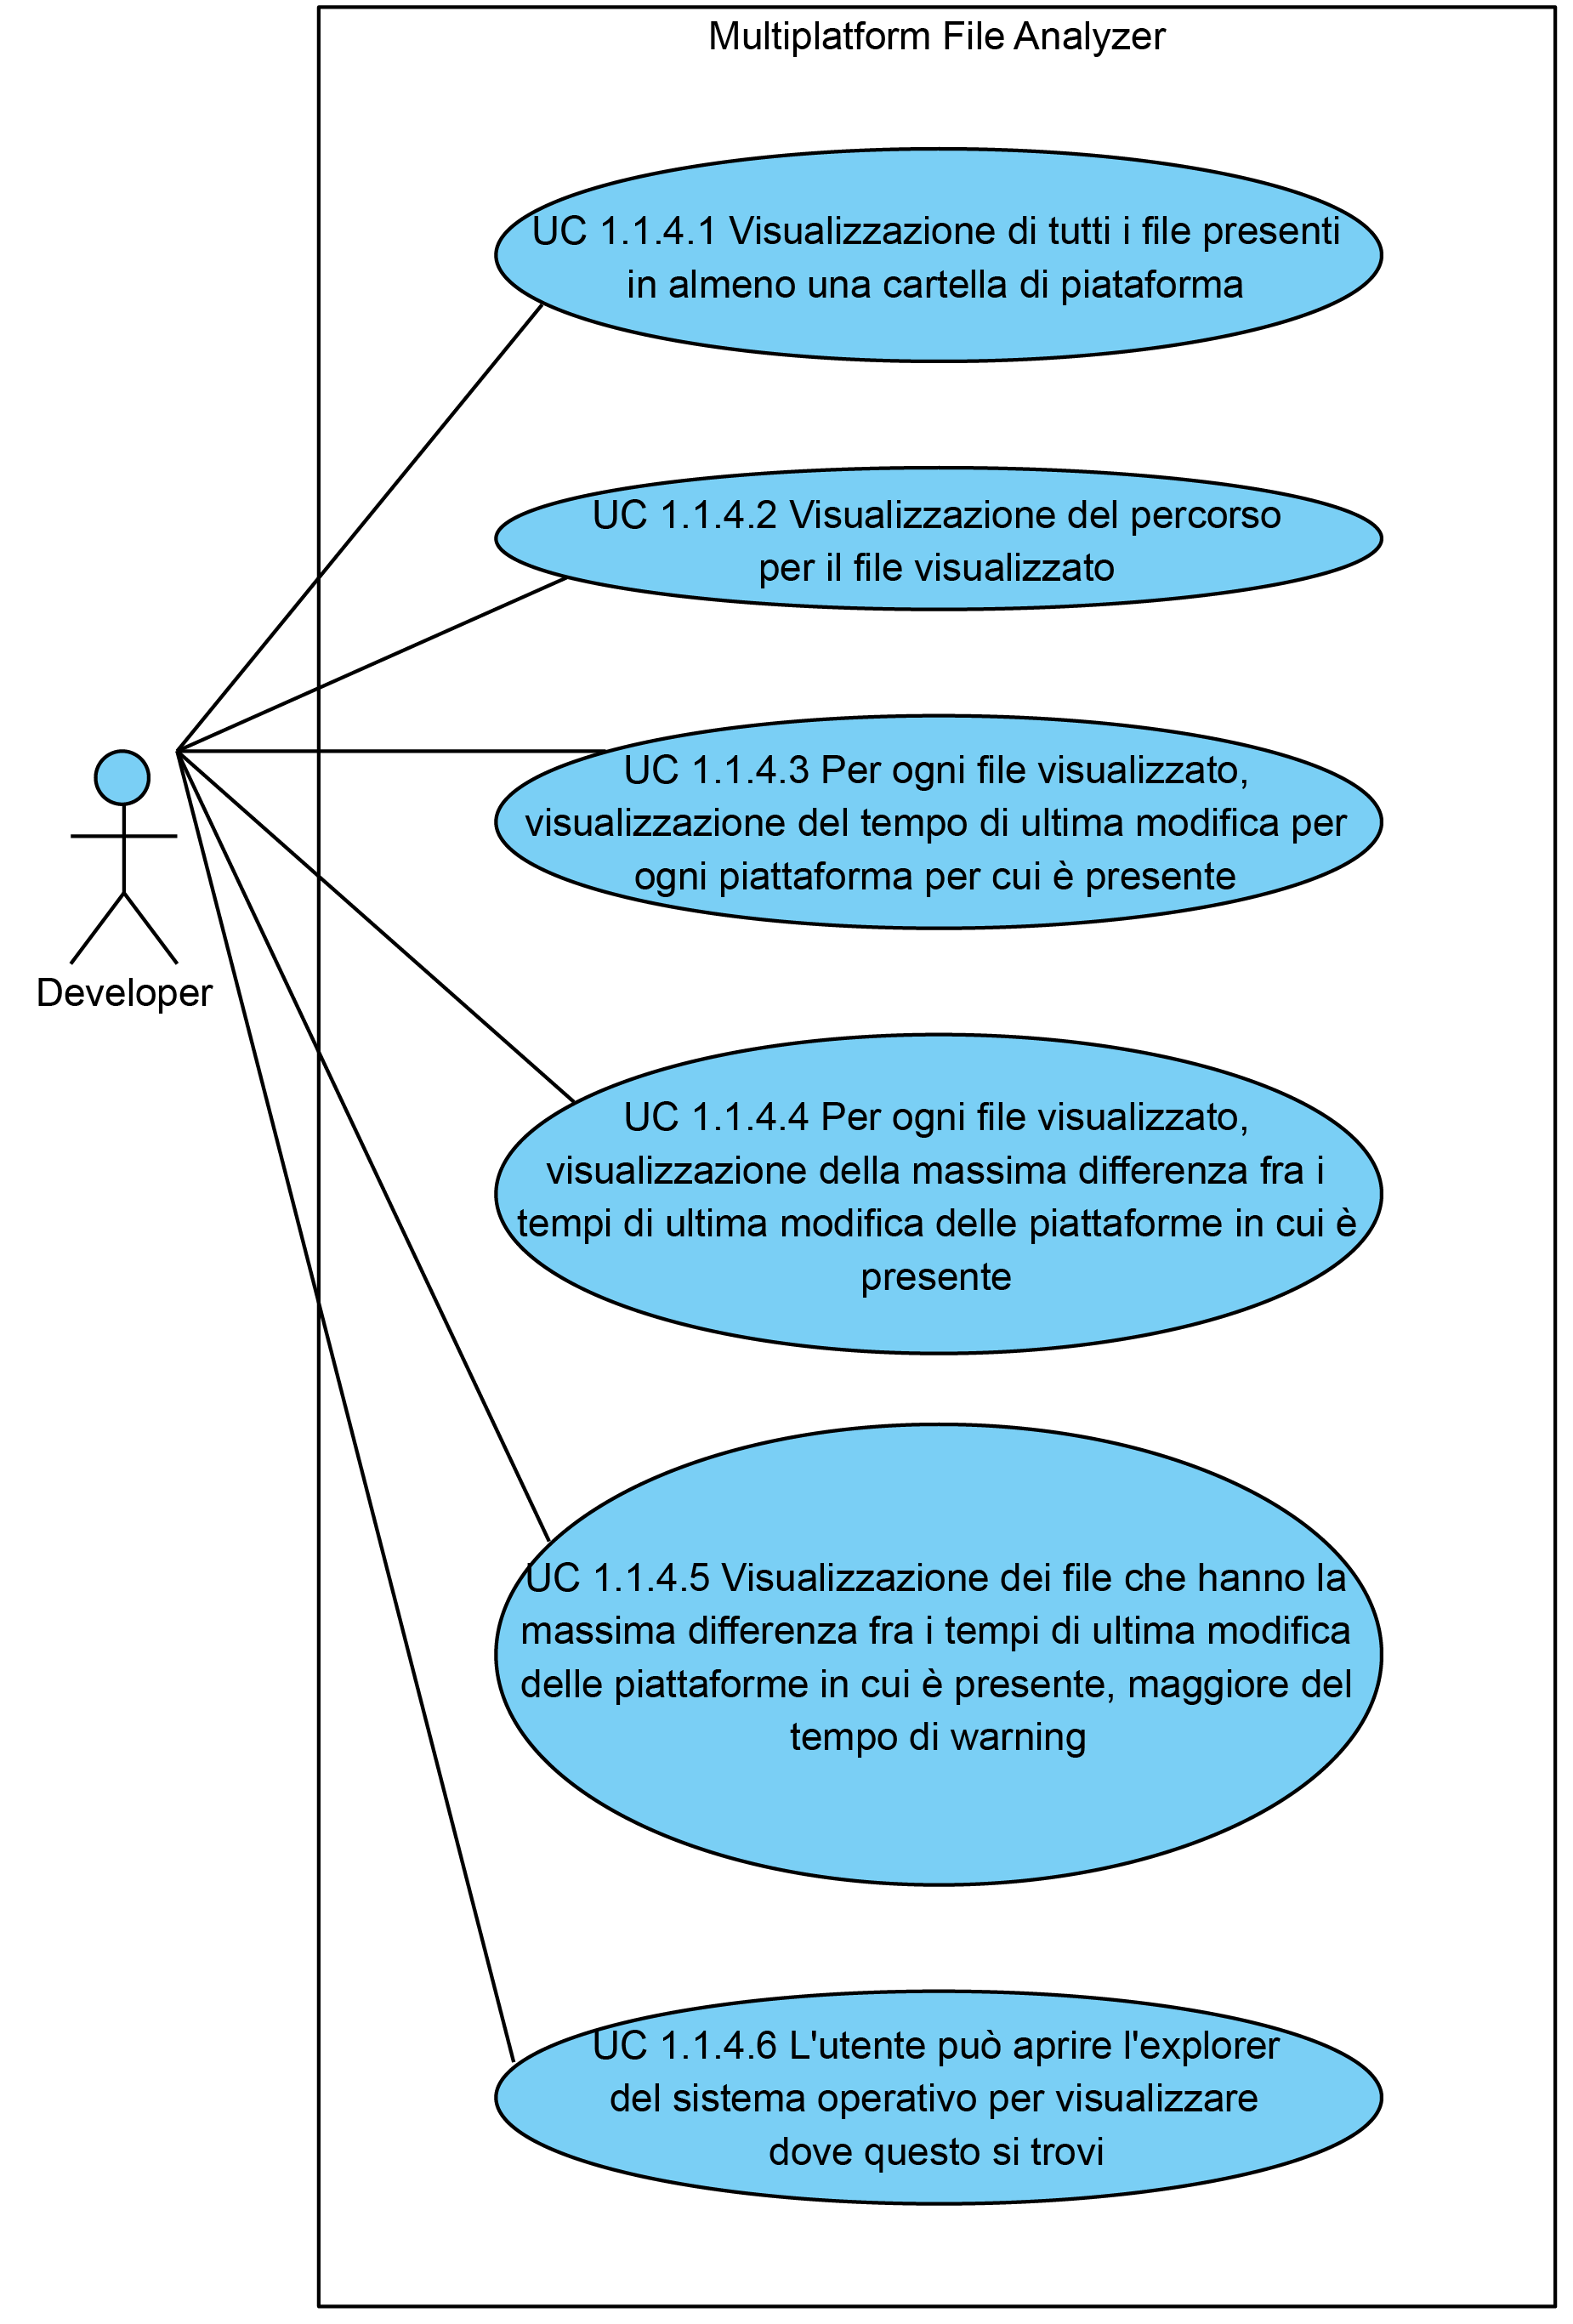
\includegraphics[width=0.9\columnwidth]{tool1/UC1-1-4.png} 
			\caption{Use Case - UC 1.1.4: Visualizzazione dei risultati dell'analisi}
		\end{figure}
		
		\begin{itemize}
			\item\textbf{Attori}: developer.
			\item\textbf{Descrizione}: un developer deve poter inserire i dati necessari all'analisi composti da un percorso di base, i nomi delle piattaforme e il tempo di warning.
			\item\textbf{Precondizione}: il developer abbia avviato l'analisi e che questa abbia terminato senza comunicare nessun errore sui dati in input.
			\item\textbf{Flusso principale degli eventi}: 
			\begin{enumerate}
				\item\textit{Visualizzazione di tutti i file presenti in almeno una cartella di piataforma} (\hyperref[subsec:UC1.1.4.1]{UC 1.1.4.1});
				
				\item\textit{Visualizzazione del percorso per il file visualizzato} (\hyperref[subsec:UC1.1.4.2]{UC 1.1.4.2});
				
				\item\textit{Per ogni file visualizzato, visualizzazione del tempo di ultima modifica per ogni piattaforma per cui è presente} (\hyperref[subsec:UC1.1.4.3]{UC 1.1.4.3});
				
				\item\textit{Per ogni file visualizzato, visualizzazione della massima differenza fra i tempi di ultima modifica delle piattaforme in cui è presente} (\hyperref[subsec:UC1.1.4.4]{UC 1.1.4.4});
				
				\item\textit{Visualizzazione dei file che hanno la massima differenza fra i tempi di ultima modifica delle piattaforme in cui è presente, maggiore del tempo di warning} (\hyperref[subsec:UC1.1.4.5]{UC 1.1.4.5});
				
				\item\textit{Il developer può aprire l'explorer del sistema operativo per visualizzare dove questo si trovi} (\hyperref[subsec:UC1.1.4.6]{UC 1.1.4.6});
				
			\end{enumerate}
			\item\textbf{Postcondizione}: i dati dell'analisi sono stati visualizzati.
		\end{itemize}

	\subsection{UC 1.1.4.1 Visualizzazione di tutti i file presenti in almeno una cartella di piataforma}
		\label{subsec:UC1.1.4.1}
		
		\begin{itemize}
			\item\textbf{Attori}: developer.
			\item\textbf{Descrizione}: il developer deve poter visualizzare tutti i file che sono stati trovati in almeno una piattaforma.
			\item\textbf{Precondizione}: il developer abbia avviato l'analisi e che questa abbia terminato senza comunicare nessun errore sui dati in input.
			\item\textbf{Scenario principale}: vengono visualizzati i file presenti in almeno una piattaforma.
			\item\textbf{Postcondizione}: il risultato dell'analisi è stato visualizzato.
		\end{itemize}
	
	\subsection{UC 1.1.4.2 Visualizzazione del percorso per il file visualizzato}
		\label{subsec:UC1.1.4.2}
	
		\begin{itemize}
			\item\textbf{Attori}: developer.
			\item\textbf{Descrizione}: il developer deve poter visualizzare il percorso del file visualizzato.
			\item\textbf{Precondizione}: il developer abbia avviato l'analisi e che questa abbia terminato senza comunicare nessun errore sui dati in input.
			\item\textbf{Scenario principale}: il developer visualizza il percorso del file visualizzato.
			\item\textbf{Postcondizione}: il percorso del file è stato visualizzato.
		\end{itemize}

	\subsection{UC 1.1.4.3 Per ogni file visualizzato, visualizzazione del tempo di ultima modifica per ogni piattaforma per cui è presente}
		\label{subsec:UC1.1.4.3}
		
		\begin{itemize}
			\item\textbf{Attori}: developer.
			\item\textbf{Descrizione}: il developer deve poter visualizzare il tempo di ultima modifica per ciascuna piattaforma in cui il file è stato trovato.
			\item\textbf{Precondizione}: il developer abbia avviato l'analisi e che questa abbia terminato senza comunicare nessun errore sui dati in input.
			\item\textbf{Scenario principale}: viene visualizzata la data di ultima modifica per ciascuna piattaforma.
			\item\textbf{Postcondizione}: il risultato dell'analisi è stato visualizzato.
		\end{itemize}
		
	\subsection{UC 1.1.4.4 Per ogni file visualizzato, visualizzazione della massima differenza fra i tempi di ultima modifica delle piattaforme in cui è presente}
		\label{subsec:UC1.1.4.4}
	
		\begin{itemize}
			\item\textbf{Attori}: developer.
			\item\textbf{Descrizione}: il developer deve poter visualizzare la massima differenza fra i tempi di ultima modifica delle piattaforme in cui è presente il file.
			\item\textbf{Precondizione}: il developer abbia avviato l'analisi e che questa abbia terminato senza comunicare nessun errore sui dati in input.
			\item\textbf{Scenario principale}: viene visualizzata la massima differenza fra i tempi di ultima modifica.
			\item\textbf{Postcondizione}: la massima differenza fra i tempi di ultima modifica è stata visualizzata.
		\end{itemize}
		
	\subsection{UC 1.1.4.5 Visualizzazione dei file che hanno la massima differenza fra i tempi di ultima modifica delle piattaforme in cui è presente, maggiore del tempo di warning}
		\label{subsec:UC1.1.4.5}
	
		\begin{itemize}
			\item\textbf{Attori}: developer.
			\item\textbf{Descrizione}: il developer deve poter visualizzare e riconoscere i file per i quali la massima differenza fra i tempi di ultima modifica è maggiore del tempo di warning.
			\item\textbf{Precondizione}: il developer abbia avviato l'analisi e che questa abbia terminato senza comunicare nessun errore sui dati in input.
			\item\textbf{Scenario principale}: vengono visualizzati tutti i file che superano il tempo di warning.
			\item\textbf{Postcondizione}: i file che superano il tempo di warning sono stati visualizzati.
		\end{itemize}
			
	\subsection{UC 1.1.4.6 L'utente può aprire l'explorer del sistema operativo per visualizzare dove questo si trovi}
		\label{subsec:UC1.1.4.6}
	
		\begin{itemize}
			\item\textbf{Attori}: developer.
			\item\textbf{Descrizione}: il developer deve poter aprire il programma che permettere l'esplorazione del file system nel punto in cui è presente il file correntemente selezionato.
			\item\textbf{Precondizione}: il developer abbia avviato l'analisi e che questa abbia terminato senza comunicare nessun errore sui dati in input.
			\item\textbf{Scenario principale}: viene visualizzato il file nella sua posizione all'interno del file system.
			\item\textbf{Postcondizione}: il file viene visualizzato nella sua posizione all'interno del file system.
		\end{itemize}


\section{Tracciamento dei requisiti}

	Partendo dai casi d'uso si è provveduto a stilare una precisa analisi dei requisiti per il tool in questione. I requisiti trovati sono stati inoltre tracciati in relazione al caso d'uso di origine.\\

	Di seguito vengono riportati tutti i requisiti individuati. Per essere più leggibili verranno separati in tabelle a seconda della loro categoria. Di ogni requisito verranno indicati: tipologia, importanza e provenienza.\\
	I requisiti dovranno essere classificati per tipo e importanza e utilizzeranno la seguente sintassi:
	\begin{center}
		R[Importanza][Tipo][Codice]
	\end{center}
	\begin{itemize}
		\item \textbf{Importanza}: può assumere solo uno fra i seguenti valori:
		\begin{itemize}
			\item \textit{0}: requisito obbligatorio;
			\item \textit{1}: requisito desiderabile;
			\item \textit{2}: requisito opzionale.
		\end{itemize}
		\item \textbf{Tipo}: pu\`{o} assumere solo uno fra i seguenti valori:
		\begin{itemize}
			\item  \textit{F}: funzionale;
			\item  \textit{Q}: di qualità;
			\item  \textit{P}: prestazionale;
			\item  \textit{V}: vincolo.
		\end{itemize}
		\item \textbf{Codice}: è il codice gerarchico univoco di ogni vincolo espresso in numeri (esempio: 1.3.2).
	\end{itemize}
	
	Per ogni requisito vengono inoltre specificati:
	\begin{itemize}
		\item \textbf{descrizione}: breve ma completa ed il \underline{meno} ambigua possibile;
		\item \textbf{fonte}: pu\`{o} essere soltanto una o pi\`{u} tra le seguenti:
		\begin{itemize}
			\item \textit{caso d'uso}: il requisito \`{e} stato estrapolato da un caso d'uso. In questo caso va indicato il codice univoco del caso d'uso. \`{E} possibile indicare come fonte pi\`{u} di un caso d'uso.
			\item \textit{interno}: è stato ritenuto giusto aggiungere questo requisito per completezza.
			\item \textit{tutor aziendale}: il requisito è stato espressamente richiesto dal tutor aziendale.
		\end{itemize}
	\end{itemize}
	
	\subsection{Requisiti funzionali}
		\begin{center}
			\begin{longtable}{p{4.2cm}!{\color{white}\vrule width 0.5mm}p{6cm}!{\color{white}\vrule width 0.5mm}p{2.5cm}!{\color{white}\vrule width 0.5mm}}
				\rowcolor{headcolor}\textcolor{white}{\textbf{Requisito}}&\textcolor{white}{\textbf{Descrizione}}&\textcolor{white}{\textbf{Fonti}}\\
				
				\rowcolor{row1}\hspace{0mm}\hypertarget{R0F1}{R0F1}  & Un utente può effettuare l'analisi dei file di un gioco multipiattaforma. & \hyperref[subsec:UC1.1]{UC 1.1}\\
				
				
				\rowcolor{row2}\hspace{2mm}\hypertarget{R0F1.1}{R0F1.1}  & L'analisi richiede l'inserimento di dati in input. & \hyperref[subsec:UC1.1.1]{UC 1.1.1}\\
				
				\rowcolor{row1}\hspace{4mm}\hypertarget{R0F1.1.1}{R0F1.1.1}  & L'analisi richiede l'inserimento di un percorso assoluto dal quale far partire l'analisi. & \hyperref[subsec:UC1.1.1.1]{UC 1.1.1.1}\\
				
				\rowcolor{row2}\hspace{4mm}\hypertarget{R0F1.1.2}{R0F1.1.2}  & L'analisi richiede l'inserimento dei nomi delle cartelle identificative di file di piattaforma. & \hyperref[subsec:UC1.1.1.2]{UC 1.1.1.2}\\
				
				\rowcolor{row1}\hspace{6mm}\hypertarget{R0F1.1.2.1}{R0F1.1.2.1}  & Il programma interpreta i nomi delle piattaforme in modo "case-insensitive". & \hyperref[subsec:UC1.1.1.2]{UC 1.1.1.2}\\
				
				\rowcolor{row2}\hspace{6mm}\hypertarget{R0F1.1.2.2}{R0F1.1.2.2}  & Il programma richiede l'inserimento dei nomi delle piattaforme come unica stringa utilizzando il carattere \sq{;} come separatore. & \hyperref[subsec:UC1.1.1.2]{UC 1.1.1.2}\\
				
				\rowcolor{row1}\hspace{4mm}\hypertarget{R0F1.1.3}{R0F1.1.3}  & L'analisi richiede l'inserimento di un tempo di warning, superato il quale, a fine l'analisi, verrà segnalato il problema se presente. & \hyperref[subsec:UC1.1.1.3]{UC 1.1.1.3}\\
				
				\rowcolor{row2}\hspace{6mm}\hypertarget{R0F1.1.3.1}{R0F1.1.3.1}  & Il formato del tempo di warning accettato prevede l'utilizzo esclusivo di numeri in formato inglese e con massimo due cifre decimali. & \hyperref[subsec:UC1.1.1.3]{UC 1.1.1.3}\\
				
				
				\rowcolor{row1}\hspace{4mm}\hypertarget{R0F1.1.4}{R0F1.1.4}  & Il programma deve memorizzare e pre-inserire i dati della precedente analisi (se esistenti) negli appositi campi per l'input dei dati, anche se tra un'analisi e la successiva il programma è stato chiuso. & Interno\\
				
				
				\rowcolor{row2}\hspace{2mm}\hypertarget{R0F1.3}{R0F1.3} & Il programma mostra gli eventuali errori sui dati in input all'analisi trovati durante l'avvio della stessa. & \hyperref[subsec:UC1.1.3]{UC 1.1.3}\\
				
				\rowcolor{row1}\hspace{4mm}\hypertarget{R0F1.3.1}{R0F1.3.1} & Il programma ferma l'avvio dell'analisi se il percorso di base non viene fornito. & \hyperref[subsec:UC1.1.3]{UC 1.1.3}\\
				
				\rowcolor{row2}\hspace{4mm}\hypertarget{R0F1.3.2}{R0F1.3.2} & Il programma ferma l'avvio dell'analisi se il percorso di base inserito non è un percorso assoluto. & \hyperref[subsec:UC1.1.3]{UC 1.1.3}\\
				
				\rowcolor{row1}\hspace{4mm}\hypertarget{R0F1.3.3}{R0F1.3.3} & Il programma ferma l'avvio dell'analisi se il percorso di base inserito non esiste nel file system. & \hyperref[subsec:UC1.1.3]{UC 1.1.3}\\
				
				\rowcolor{row2}\hspace{4mm}\hypertarget{R0F1.3.4}{R0F1.3.4} & Il programma ferma l'avvio dell'analisi se il contenuto del percorso di base inserito non è leggibile. & \hyperref[subsec:UC1.1.3]{UC 1.1.3}\\
				
				
				\rowcolor{row1}\hspace{2mm}\hypertarget{R0F1.4}{R0F1.4} & Il programma permette la visualizzazione dei dati output dell'analisi. & \hyperref[subsec:UC1.1.4]{UC 1.1.4}\\
				
				\rowcolor{row2}\hspace{4mm}\hypertarget{R0F1.4.1}{R0F1.4.1} & Nell'output dell'analisi è presente ciascun file presente in almeno un cartella di piattaforma. & \hyperref[subsec:UC1.1.4.1]{UC 1.1.4.1}\\
				
				\rowcolor{row1}\hspace{4mm}\hypertarget{R0F1.4.2}{R0F1.4.2} & Per ciascun file presente nell'output è visibile la data di ultima modifica per ciascuna piattaforma in cui è presente. & \hyperref[subsec:UC1.1.4.2]{UC 1.1.4.2}\\
				
				\rowcolor{row2}\hspace{4mm}\hypertarget{R0F1.4.3}{R0F1.4.3} & Per ciascun file presente nell'output è indicato il percorso di relativo a partire dal percorso di base inserito in input all'analisi. & \hyperref[subsec:UC1.1.4.3]{UC 1.1.4.3}\\
				
				\rowcolor{row1}\hspace{4mm}\hypertarget{R0F1.4.4}{R0F1.4.4} & Per ciascun file presente nell'output è indicato il nome del file completo di estensione. & \hyperref[subsec:UC1.1.4.4]{UC 1.1.4.4}\\
				
				\rowcolor{row2}\hspace{4mm}\hypertarget{R0F1.4.5}{R0F1.4.5} & Per ciascun file presente nell'output è indicata la massima differenza tra le date di ultima modifica delle piattaforme per cui è presente & \hyperref[subsec:UC1.1.4.5]{UC 1.1.4.5}\\
				
				\rowcolor{row1}\hspace{6mm}\hypertarget{R0F1.4.5.1}{R0F1.4.5.1} & Se il tempo massimo per ciascuno file è superiore al tempo di warning inserito in input allora questo viene evidenziato come warning. & \hyperref[subsec:UC1.1.4.5]{UC 1.1.4.5}\\
				
				\rowcolor{row2}\hspace{6mm}\hypertarget{R0F1.4.5.2}{R0F1.4.5.2} & Il tempo è mostrato nella stessa unità di misura in cui è stato inserito il tempo di warning. & \hyperref[subsec:UC1.1.4.5]{UC 1.1.4.5}\\
				
				\rowcolor{row1}\hspace{4mm}\hypertarget{R0F1.4.6}{R0F1.4.6} & Il programma permette di aprire il programma per esplorare il file system di defalut del sistema e visualizzare la cartella dove è presente il file & \hyperref[subsec:UC1.1.4.6]{UC 1.1.4.6}\\
				
				\hline
				\caption{Requisiti funzionali}
			\end{longtable}
		\end{center}

	\subsection{Requisiti di qualità}
		\begin{center}
			\begin{longtable}{p{4.2cm}!{\color{white}\vrule width 0.5mm}p{6cm}!{\color{white}\vrule width 0.5mm}p{2.5cm}!{\color{white}\vrule width 0.5mm}}
				\rowcolor{headcolor}\textcolor{white}{\textbf{Requisito}}&\textcolor{white}{\textbf{Descrizione}}&\textcolor{white}{\textbf{Fonti}}\\
				
				\rowcolor{row1}\hspace{0mm}\hypertarget{R0Q1}{R0Q1} & Viene fornito insieme al programma un l'help con la guida alla compilazione e al deploy per sistemi Windows. & Tutor interno\\
				
				\rowcolor{row2}\hspace{0mm}\hypertarget{R0Q2}{R0Q2} & Viene fornito un l'help che spiega come utilizzare il programma. & Tutor interno\\
				
				\hline
				\caption{Requisiti di vincolo}
			\end{longtable}
		\end{center}

	\subsection{Requisiti di vincolo}
		\begin{center}
			\begin{longtable}{p{4.2cm}!{\color{white}\vrule width 0.5mm}p{6cm}!{\color{white}\vrule width 0.5mm}p{2.5cm}!{\color{white}\vrule width 0.5mm}}
				\rowcolor{headcolor}\textcolor{white}{\textbf{Requisito}}&\textcolor{white}{\textbf{Descrizione}}&\textcolor{white}{\textbf{Fonti}}\\
				
				\rowcolor{row1}\hspace{0mm}\hypertarget{R0V1}{R0V1} & Il programma deve funzionare su Windows 7 SP1 32 e 64 bit. & Tutor interno\\
				
				\rowcolor{row2}\hspace{0mm}\hypertarget{R0V2}{R0V2} & Il programma deve essere scritto utilizzando il linguaggio C++ 98. & Tutor interno\\
				
				\hline
				\caption{Requisiti di vincolo}
			\end{longtable}
		\end{center}
		
\section{Tecnologie e strumenti}
	Di seguito viene fornita una panoramica delle tecnologie e strumenti utilizzati per lo sviluppo di Multiplatform File Analyzer.
	
	\subsection{Qt Framework}
		Per lo sviluppo del tool è stato usato Qt Framework versione 5.3.1. Qt è un potente Framework multipiattaforma che offre una vastissima serie di librerie di utilità, grazie alle quali lo sviluppo diviene agevole e veloce, permettendo quasi  sempre di non legarsi a specifiche implementazioni per piattaforma.\\
		In particolare è stata usata la libreria per costruire le interfacce grafiche e la libreria per accedere al file system e leggerne le informazioni.
		
	\subsection{Qt Creator}
		Come IDE per lo sviluppo ci si è affidati a Qt Creator 3.1.2. IDE semplice e performante che si integra perfettamente con il mondo Qt, offrendo addirittura la consultazione veloce della documentazione direttamente nell'IDE.
		
\section{Ciclo di vita del software}
	Essendo Multiplatform File Analyzer uno strumento di piccole dimensioni si è adottato un semplice modello di ciclo di vita incrementale, con un singolo incremento corrispondente alla consegna finale.
	
\section{Progettazione}
	Il software è stato progettato per offrire una semplice espandibilità, allo scopo la strutturazione generale segue il collaudato Design Pattern \textit{MVC}, dove trovano luogo i seguenti pacchetti: \texttt{controller}, \texttt{view} e \texttt{data}. È inoltre presente il pacchetto \texttt{core} in cui è inserita l'implementazione degli algoritmi di business del tool, ad esempio l'algoritmo che esegue l'analisi.\\
	
	Il pacchetto core è implementato con il Design Pattern \textit{Strategy} allo scopo di permettere una facile estensione o sostituzione dell'algoritmo che esegue l'analisi, anche a run-time.\\
	
	Per permettere una facile e veloce connessione tra gli stati descritti dall'\textit{MVC} è stato adottato il Design Pattern \textit{Observer}, implementato nell'omonimo pacchetto \textit{observer}.\\
	
	È stato scelto di utilizzare il Design Pattern \textit{Strategy} per rendere modificabile facilmente l'implementazione dell'algoritmo che effettua l'analisi, all'interno del pacchetto \texttt{core}.\\
	
	È stato inoltre cercato di utilizzare le classi del Framework Qt in modo isolato alle sole parti strettamente necessarie, ovvero la GUI e l'analisi del file system. Questo allo scopo di rendere il tool slegato dalle implementazioni specifiche, in favore di una più semplice espandibilità.
	
	\subsection{Diagramma delle classi}
		Di seguito è presente il diagramma delle classi espresso tramite il formalismo UML 2.0. Nel diagramma è inoltre possibile vedere le principali dipendenza verso le classi del Framework Qt.
		
		\begin{figure}[!h] 
			\centering 
			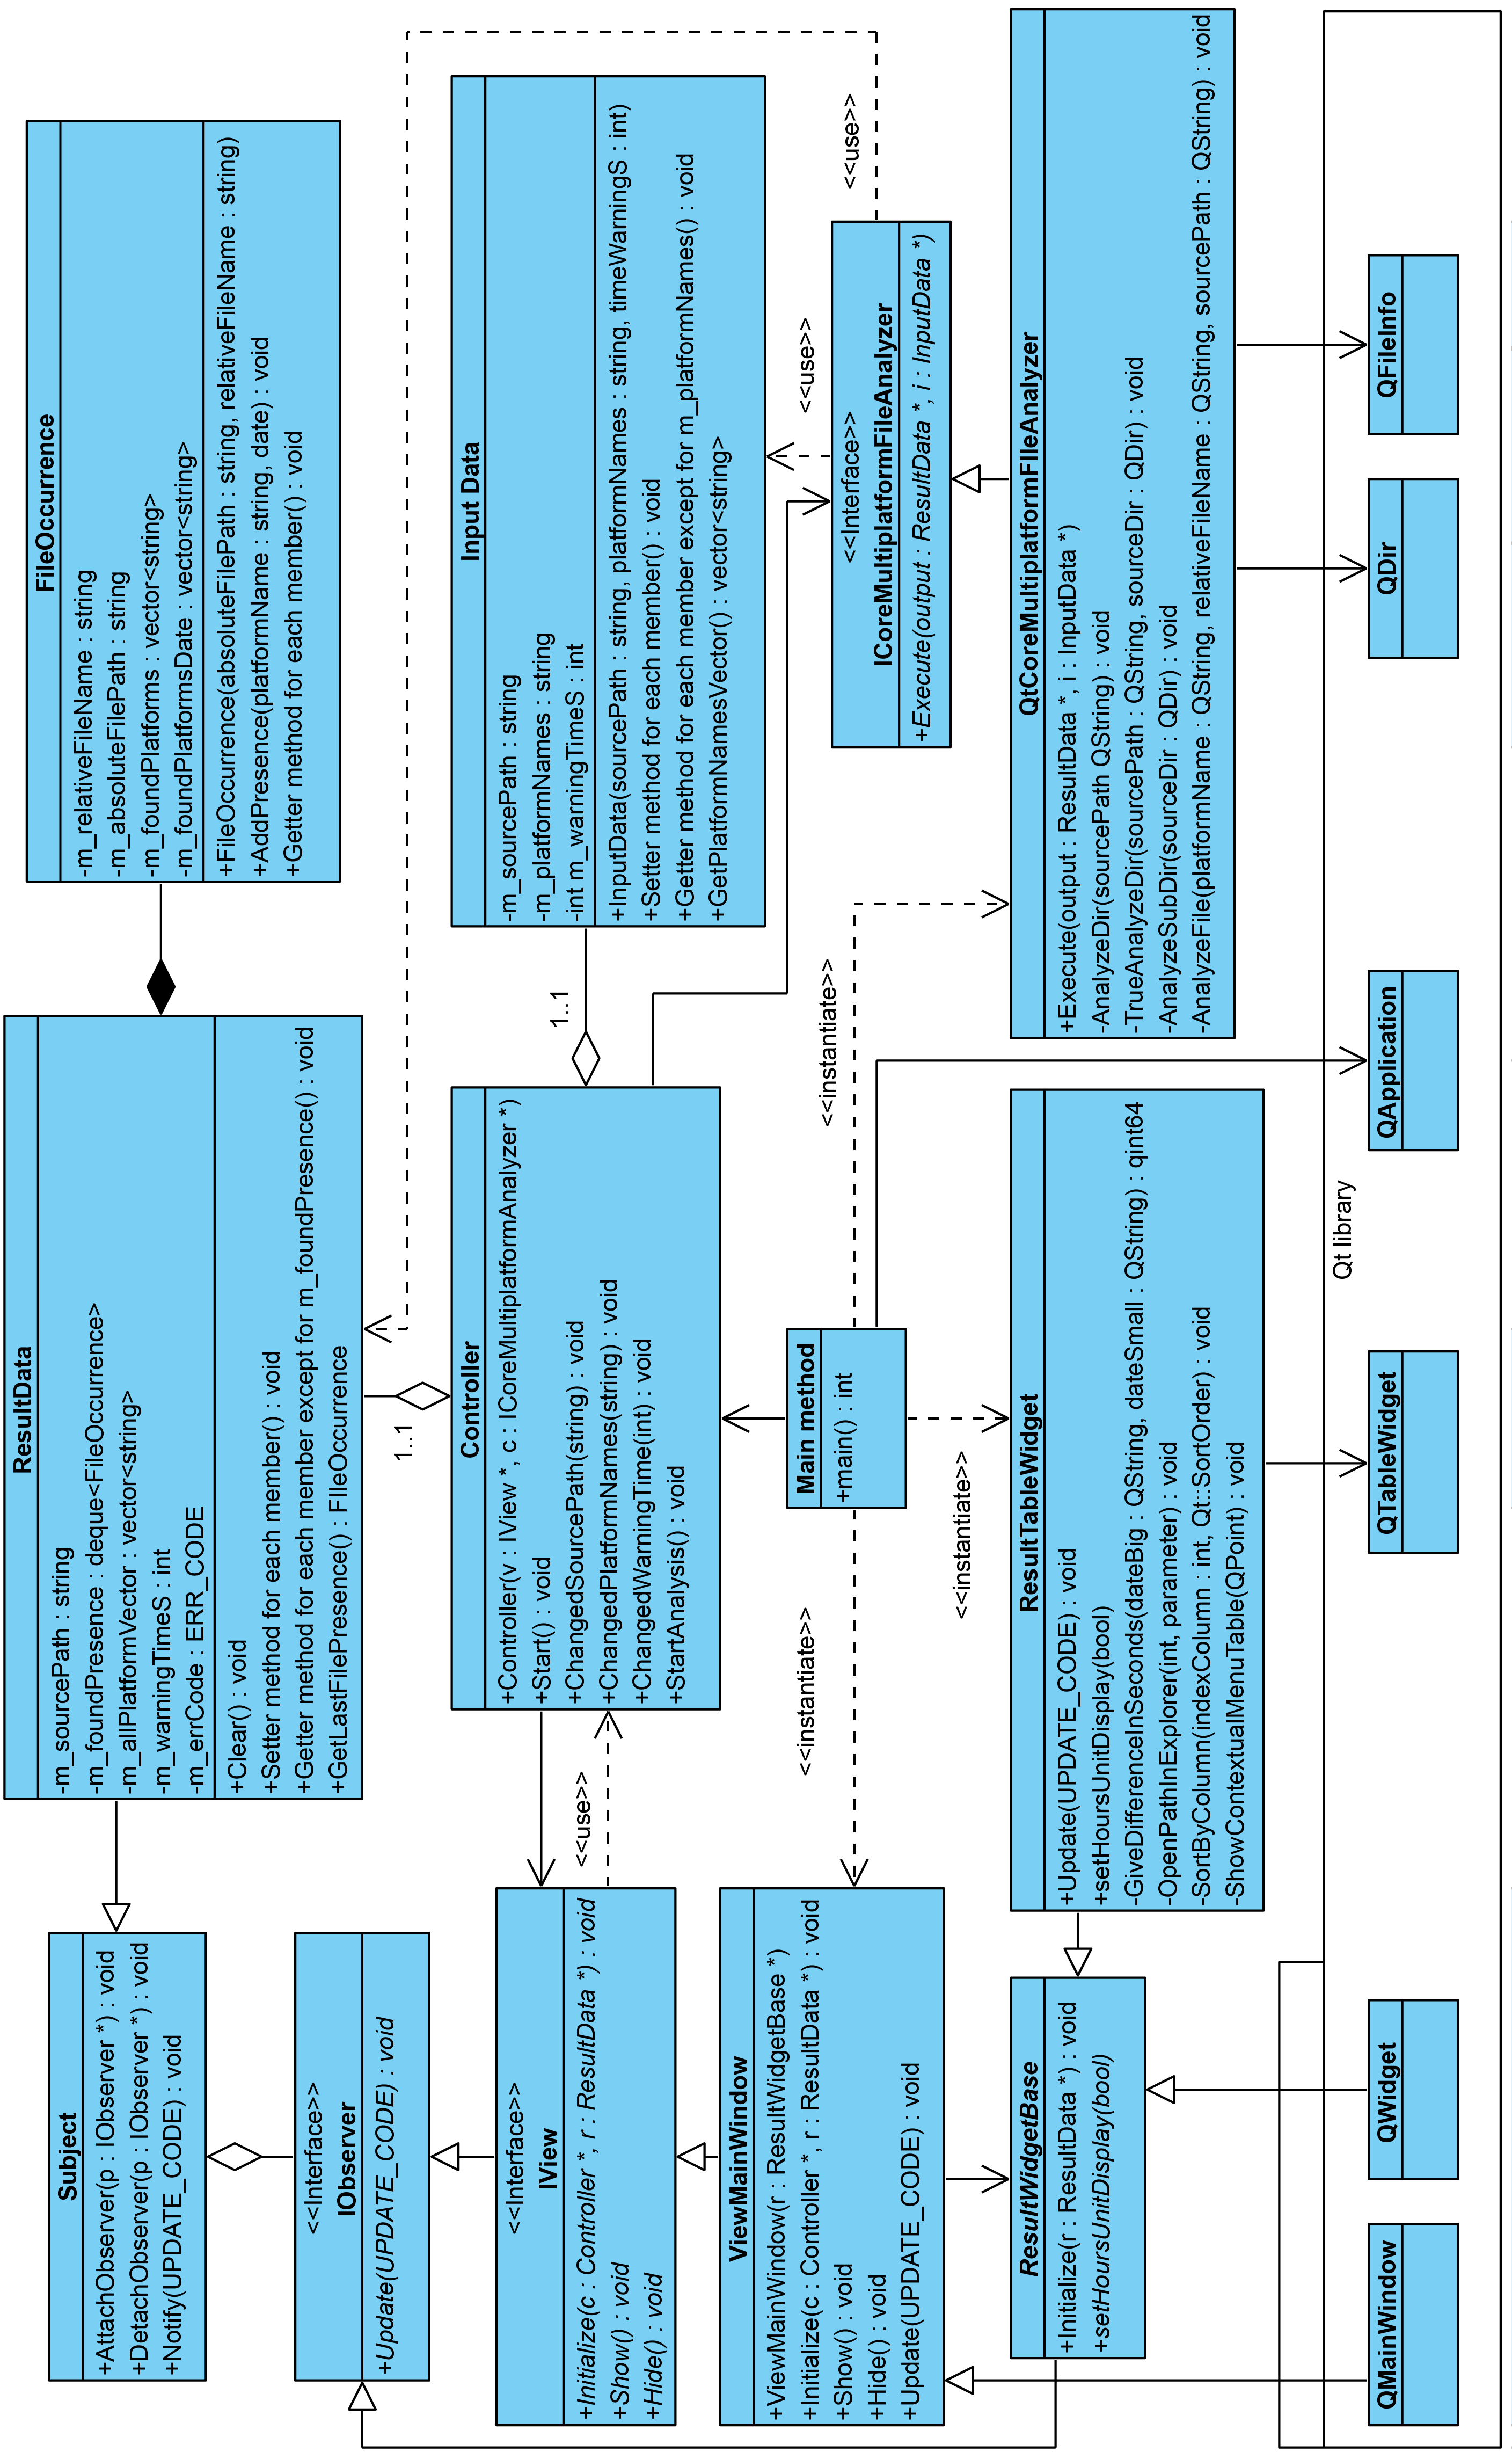
\includegraphics[width=0.98\columnwidth]{tool1/Tool-1-Diagramma-Classi.png} 
			\caption{Diagramma delle classi di Multiplatform File Analyzer}
		\end{figure}
	
		\newpage
	
	\subsection{Pacchetto controller}
		Il pacchetto è composto dalla sola classe \texttt{Controller} che svolge il compito di controllore del sistema. È questo il solo pacchetto utilizzato dall funzione \texttt{main}.
		
		\subsubsection{Classe Controller}
			La classe \texttt{Controller} si occupa di avviare il sistema. Essa provvede ad allocare tutti gli oggetti necessari e al relativo rilascio al termine del programma. Inoltre seleziona la view e la connette con le classi che rappresentano i dati. Infine raccoglie i comandi utente provenienti dalla view e li esegue grazie al pacchetto \texttt{core}.
	
	\subsection{Pacchetto observer}
		Questo pacchetto rappresenta l'implementazione del Design Pattern \textit{Observer} ed è stato utilizzato per tenere aggiornata la view al cambiamento dei dati.
		
		\subsubsection{Interfaccia IObserver}
		\texttt{IObserver} è l'interfaccia che rappresenta gli oggetti che osservano le modifiche di altri oggetti. Essa contiene il metodo virtuale puro \texttt{Update} che i soggetti osservati invocano per segnalare il fatto che sono stati modificati e che quindi un aggiornamento è necessario. Le classi concrete che avranno la necessità di osservare un soggetto deriveranno da \texttt{IObserver} implementando il metodo \texttt{Update}.
		
		\subsubsection{Classe Subject}
		La classe \texttt{Subject} rappresenta un soggetto che può essere osservato. Essa contiene il codice necessario per notificare tutti gli osservatori dell'avvenuto cambiamento. Mantiene inoltre una lista degli osservatori da notificare, i quali possono iscriversi se desiderano ricevere la notifica, oppure rimuoversi se non è più necessario ricevere aggiornamenti. Le classi che devono essere osservate deriveranno da questa.
	
	\subsection{Pacchetto data}
		Il pacchetto \texttt{data} contiene tutte le classi che rappresentano i dati di business del programma. Allo scopo di rendere il programma eseguibile anche su un semplice terminale e quindi disaccoppiato dal mondo Qt, le classi di dati sono state implementate con la Standard Template Library (STL), piuttosto che le classi collezione offerte dal framework in uso.
	
		\subsubsection{Classe InputData}
			La classe \texttt{InputData} raccoglie tutti i dati che sono di input all'analisi. Contiene quindi il percorso di partenza, i nomi delle piattaforme ed il tempo di warning. È questa classe che si occupa della trasformazione della stringa contenente tutte le piattaforme in un \texttt{Vector}.
				
		\subsubsection{Classe FileOccurrence}
			La classe \texttt{FileOccurrence} rappresenta un file trovato in almeno una cartella di piattaforma durante l'analisi. Per il file trovato, la classe contiene il percorso assoluto, il nome, tutte le piattaforme in cui è stato trovato e, per ciascuna, la data di ultima modifica. 
				
		\subsubsection{ResultData}
			La classe \texttt{ResultData} contiene tutti i dati presenti come output di una analisi. Contiene quindi una collezione di \texttt{FileOccurrence} e tutti i dati di input all'analisi.\\
			Essa deriva dalla classe \texttt{Subject} per permettere ad un osservatore, tipicamente un elemento dell View, di aggiornarsi al variare dei risultati. Permettendo di mostrare i risultati dell'analisi in modo interattivo durante l'inserimento di ogni nuovo \texttt{FileOccurence} trovato.
			
	\subsection{Pacchetto view}
		Questo pacchetto si occupa delle interfacce utente, derivando e personalizzando le classi offerte dal Framework Qt.
		
		\subsubsection{Iterfaccia IView}
			\texttt{IView} è una classe astratta che rappresenta una generica view.
			
		\subsubsection{Classe ViewMainWindow}
			La classe \texttt{ViewMainWindow} implementa \texttt{IView} tramite una finestra. Eredita e specializza la classe \texttt{QMainWindow} di Qt. Raccoglie i comandi utente e ne delega l'esecuzione al controller.
			
		\subsubsection{Classe ResultWidgetBase}
			La classe astratta \texttt{ResultWidgetBase} rappresenta un generico widget integrabile in una interfaccia grafica che sfrutta le classi del Framework Qt per la visualizzazione dell'output dell'analisi.
			
		\subsubsection{Classe ResultTableWIdget}
			La classe \texttt{ResultWidget} implementa la classe base astratta \texttt{ResultWidgetBase} mostrando l'output dell'analisi in forma tabellare, dedicando una riga a ciascun file trovato.
			
	\subsection{Core}
		Il pacchetto si occupa della realizzazione dell'analisi e di tutti gli algoritmi di business del tool. Utilizza il Design Pattern \textit{Strategy} per l'organizzazione delle classe contenute.
		
		\subsubsection{Interfaccia ICoreMultiplatformFileAnalyzer}
			\texttt{ICoreMultiplatformFileAnalyzer} rappresenta l'algoritmo di business del programma, ovvero quello che effettua l'analisi e riempie un'istanza della classe \texttt{ResultData} con il risultato.
			
		\subsubsection{Classe QtCoreMultiplatformFIleAnalyzer}
			La classe \texttt{QtCoreMultiplatformFIleAnalyzer} implementa l'interfaccia\\ \texttt{ICoreMultiplatformFileAnalyzer} utilizzando il Framework Qt per esplorare il file system.
			
\section{Codifica}
	Tutto il codice del tool è stato pubblicato sulla piattaforma GitHub, accedibile tramite il seguente indirizzo: \url{https://github.com/Mauxx91/Multiplatform-File-Analyzer}. Tutto il codice è disponibile gratuitamente sotto licenza GNU GPL v3\footnote{Un approfondimento sulla licenza può essere trovato al seguente indirizzo: \url{http://www.gnu.org/copyleft/gpl.html}.}\\

	Tutto il codice è stato scritto in lingua inglese, compresi i commenti, dei quali si è cercato di scriverne il più possibile.
	La codifica ha seguito alcune convenzioni della famosa notazione Ungherese. Di seguito sono elencati i formalismi utilizzati nel codice:
	
	\begin{itemize}
		\item \textbf{prefissi:}
		\begin{itemize}
			\item \textbf{m}: usato per le variabili membro (esempio: \texttt{m\_keyName});
			\item \textbf{p}: usato per le variabili puntatore (esempio: \texttt{m\_pkeyNameList});
			\item \textbf{o}: usato per le variabili input alla funzione che sono usate come output (esempio: \texttt{o\_foundKeys});
			\item \textbf{I}: usato per le classi interfacce (esempio: \texttt{IObserver}).
		\end{itemize}
		\item \textbf{suffissi:}
		\begin{itemize}
			\item \textbf{Base}: usato per le classi astratte (esempio: \texttt{ResultWidgetBase});
		\end{itemize}
		\item \textbf{capitalizzazione:}
		\begin{itemize}
			\item \textbf{variabili e parametri}: iniziano sempre in minuscolo e usano una lettera minuscola per ogni parola (esempio: \texttt{m\_parentWidget}, \texttt{returnValue});
			\item \textbf{macro ed enum}: completamente in maiuscolo con le diverse parole separate dal carattere \sq{\_} (esempio: \texttt{UPDATE\_CODE});
			\item \textbf{classi, funzioni e metodi}: iniziano sempre in maiuscolo e ogni parola diversa parte in maiuscolo (esempio: \texttt{FileOccurrence});
		\end{itemize}
	\end{itemize}
	
	todo -> include del codice o no?
	
\section{Conclusioni}
	Tutti i requisiti sono stati soddisfatti come pianificato e nei tempi prestabiliti.\\
	La realizzazione del tool ha messo di fronte lo studente a una problematica reale presente durante lo sviluppo di giochi multipiattaforma. Contemporaneamente gli ha permesso di interfacciarsi ai comuni problemi legati alla manutenzione dei moltissimi file presenti nei grandi progetti, lasciandogli la libertà di progettare e realizzare una soluzione.\\
	Lo studente ha inoltre approfondito le tematiche della creazione di interfacce usabili e degli algoritmi per l'esplorazione del file system.